%\documentclass[10pt,slidestop,mathserif]{beamer}
\documentclass[10pt,handout,mathserif]{beamer}
%\documentclass[handout,10pt,slidestop,mathserif]{beamer}
\usetheme{Madrid}
\usecolortheme{seahorse}

\usepackage{tabularx}
\usepackage{verbatim}
\usepackage{graphics}
\usepackage{graphicx}
\usepackage{Sweave}
\usepackage{moreverb}
\usepackage{pgf}
\usepackage{tikz}
\usepackage[notocbib]{apacite}
\usepackage{MnSymbol}


\newcommand{\putat}[3]{\begin{picture}(0,0)(0,0)\put(#1,#2){#3}\end{picture}}
  
\newenvironment{changemargin}[2]{%
  \begin{list}{}{%
    \setlength{\topsep}{0pt}%
    \setlength{\leftmargin}{#1}%
    \setlength{\rightmargin}{#2}%
    \setlength{\listparindent}{\parindent}%
    \setlength{\itemindent}{\parindent}%
    \setlength{\parsep}{\parskip}%
  }%
  \item[]}{\end{list}}

%% Define a new 'leo' style for the package that will use a smaller font.
\makeatletter
\def\url@leostyle{%
  \@ifundefined{selectfont}{\def\UrlFont{\sf}}{\def\UrlFont{\tiny\ttfamily}}}
\makeatother

\title[Dissertation Proposal]{A National Study Comparing Charter and Traditional Public Schools Using Propensity Score Analysis}
\subtitle{Dissertation Defense}
\author[Bryer]{Jason M. Bryer}
\institute[University at Albany]{School of Education\\
Department of Educational \& Counseling Psychology\\
Division of Educational Psychology \& Methodology\\
University at Albany}
\date{September 8, 2014}

\begin{document}


\frame{\titlepage}


%%%%%%%%%%%%%%%%%%%%%%%%%%%%%%%%%%%%%%%%%%%%%%%%%%%%%%%%%%%%%%%%%%%%%%%%%%%%%%%%
%\section{Acknowledgements}
\begin{frame}[c]
    \begin{center}\Large It takes a village...\\
    \pause to complete a dissertation!\end{center}
\end{frame}

\setbeamercovered{transparent}


%%%%%%%%%%%%%%%%%%%%%%%%%%%%%%%%%%%%%%%%%%%%%%%%%%%%%%%%%%%%%%%%%%%%%%%%%%%%%%%%
\frame{\frametitle{Outline}\tableofcontents}

%%%%%%%%%%%%%%%%%%%%%%%%%%%%%%%%%%%%%%%%%%%%%%%%%%%%%%%%%%%%%%%%%%%%%%%%%%%%%%%%
\section{Overview}

\subsection{What are Charter Schools?}

\begin{frame}
	\frametitle{What are Charter Schools?}
	The first charter school opened in Minnesota in 1991
	In principle, charter schools have opted out of bureaucratic rules and union contracts in order to gain academic autonomy. The standard argument has become that this autonomy will lead to higher student test scores and better academic environments \cite{Wells2002}. The idea is that, under the charter framework, teachers, administrators, students and the community that comprise the charter school would be free to innovate
	
	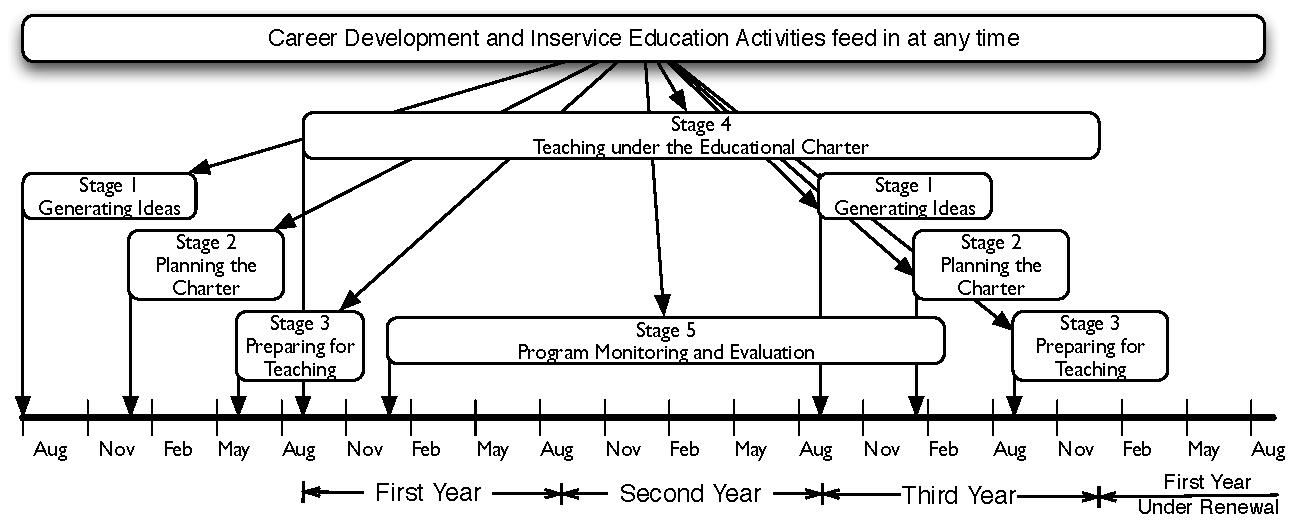
\includegraphics[width=\textwidth,keepaspectratio=true]{../Figures/Timeline.pdf}
	
	\footnotesize Adapted from Budde (1988).
\end{frame}

\begin{frame}[c]
	\frametitle{Growth in Number of Charter Schools}
	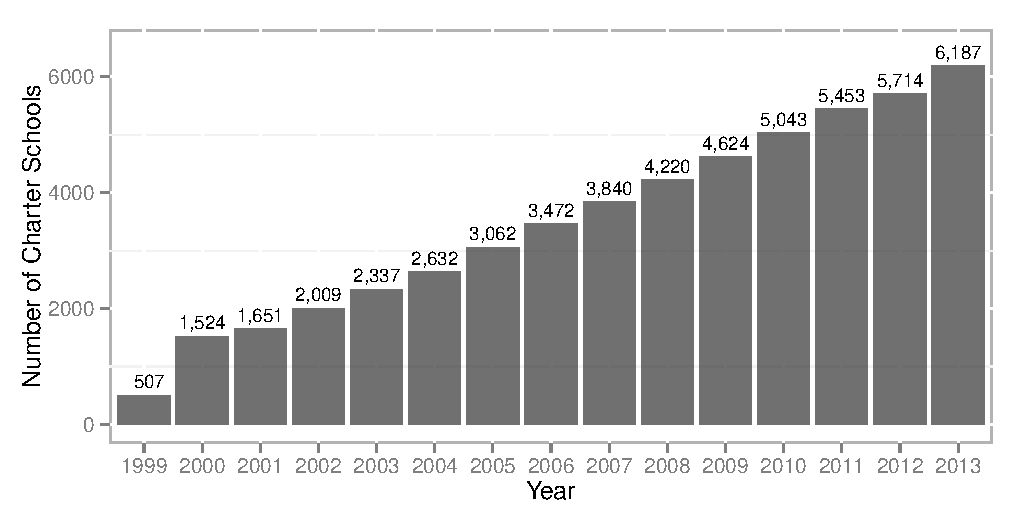
\includegraphics[width=\textwidth,keepaspectratio=true]{../Figures/CharterSchoolGrowth.pdf}
\end{frame}

\subsection{Literature Review}

\begin{frame}[c]
	\frametitle{National Studies Examining Charter and Traditional Public Schools}
	The number of studies that consider charter school effectiveness from a national perspective are limited.
	\ \\
	\begin{enumerate}
	    \setlength{\itemsep}{10pt}
		\item \citeA{BraunJenkinsGrigg2006} examined charter and traditional public schools using hierarchal linear modeling (HLM) with NAEP 2005. They found that there was often no difference, and in some instances charter school students performed worse.
		\pause
		\item \textit{The CREDO Study} - \citeA{credo} conducted a study of more than 1.7 million records from 2400 charter within 16 states. The methodology involves creating a Virtual Control Record (VCR) for each charter school student which is used to find matching student from an eligible traditional public school.
		Overall results show that charter school students performed, on average, 0.01 and 0.03 standard deviations below public school students for reading and math, respectively.
	\end{enumerate}
\end{frame}

%\begin{frame}[c]
%\begin{quote}    %Good quote... come back to the idea at some point!
%If, however, charter schools are not improving the achievement of disadvantaged children, it may be that the cause of low student performance is not bureaucratic rules but something else. When a treatment is based on a diagnosis, and the treatment doesn't work, it is prudent to examine not only whether the treatment should be improved, but also whether the diagnosis might be flawed. \cite{Carnoy2005}
%\end{quote}
%\end{frame}

\subsection{Issues with Charter Schools}

\begin{frame}[c]
	\frametitle{Issues with Charter Schools Research}
	\begin{enumerate}[<+-| alert@+>]
	    \setlength{\itemsep}{15pt}
		\item The issue of selection bias
		\item The variation in types or kinds of charter schools.
		\item The nature of student achievement. Research has shown there are numerous factors that contribute to student success including, but not limited to, social economic status, parental education, motivation, etc. The ability to decipher how school choice contributes to student learning in the context of all the other factors cannot help but be difficult.
	\end{enumerate}
	\ \\\ \\
	\pause
	A fourth issue not cited by \citeA{BettsHill2006} is the role of charter school laws.
\end{frame}

\subsection{Research Question}

\begin{frame}[c]
	\frametitle{Research Questions}
	\citeA{BettsHill2006} outline three major issues with charter school research:
	\begin{enumerate}[<+-| alert@+>]
    \setlength{\itemsep}{15pt}
	\item Given appropriate adjustments based on available student data, is there a discernible difference between charter and traditional public schools with regard to math and reading scores on the NAEP scores at grades 4 and 8?
    \item If so, what is the nature and magnitude of this difference for the two outcomes, reading and mathematics scores?
    \item What is the relationship, if any, of different charter school laws on charter school student performance in math and reading at grades 4 and 8?
	\end{enumerate}
\end{frame}

%%%%%%%%%%%%%%%%%%%%%%%%%%%%%%%%%%%%%%%%%%%%%%%%%%%%%%%%%%%%%%%%%%%%%%%%%%%%%%%%
\section{Method}

\subsection{Propensity Scores}

\begin{frame}
	\frametitle{Propensity Scores}
    Propensity scores are the ``conditional probability of being in the treatment" \cite{RosenbaumRubin1983}, defined as:
    
    \begin{equation}
    \pi ({ X }_{ i }) \; \equiv \; Pr({ T }_{ i } = 1 | { X }_{ i })
    \end{equation}
    \pause
    
    Let $X$ is a matrix of observed covariates. The balancing property under exogeneity states that,

    \begin{equation}
    { T }_{ i } \; \upModels { X }_{ i } \;| \; \pi ({ X }_{ i })
    \end{equation}
    
    \pause
    For randomized experiments, the strong ignobility assumption states,

    \begin{equation}
    ({ Y }_{ i }(1),{ Y }_{ i }(0)) \; \upModels \; { T }_{ i }|{ X }_{ i }
    \end{equation}

    for all ${X}_{i}$. That is, treatment is independent of all covariates, observed or otherwise. 
    
    \pause
    However, the strong ignobility assumption can be restated with the propensity score as,

    \begin{equation}
    ({ Y }_{ i }(1),{ Y }_{ i }(0)) \; \upModels \; { T }_{ i } \; | \; \pi({ X }_{ i })
    \end{equation}

\end{frame}

\subsection{Methods used for this Study}

\begin{frame}
	\frametitle{Propensity Score Methods for this Study}
	\begin{enumerate}
	    \setlength{\itemsep}{15pt}

		\item \textit{Propensity score analysis using stratification.}
		\begin{enumerate}
			\item Full logistic regression. 
			\item Logistic regression with step AIC.
			\item Conditional inference trees \cite{HorthornHornikZeileis2006}.
		\end{enumerate}
	\pause
	\item \textit{Propensity score matching.} 
		\begin{enumerate}
			\item One-to-one
			\item One-to-five
			\item One-to-ten.
		\end{enumerate}
		A dependent sample analysis will be performed on the resulting matched pairs \cite{Austin2011}.
	\pause
	\item \textit{Multilevel propensity score analysis.}
		\begin{enumerate}
			\item Full logistic regression.
			\item Logistic regression with step AIC.
			\item Conditional inference trees.
		\end{enumerate}
	\end{enumerate}
\end{frame}

\subsection{The \texttt{multilevelPSA} R Package}

\begin{frame}
    \frametitle{The \texttt{multilevelPSA} Package}
    \begin{itemize}
        \setlength{\itemsep}{10pt}
        \item The \texttt{multilevelPSA} R package was written to perform the analysis and generate the figures used for this dissertation.
        \item Currently available from the Comprehensive R Archive Network (CRAN) at \url{http://cran.r-project.org/web/packages/multilevelPSA/index.html}
        \item Contains 16 functions, 4 demos, and a vignette. Examples utilize the Programme of International Student Assessment (PISA) examining the differences between private and public schools internationally.
    \end{itemize}
\end{frame}


\begin{frame}[c]
	\frametitle{National Assessment of Educational Progress (NAEP)}
	\begin{itemize}
    \setlength{\itemsep}{10pt}
	\item Congressionally mandated.
	\item Started in 1971.
	\item Provides national measures of student achievement in many subjects including mathematics, reading, science, writing, history, civics, and the arts.
	    \item Used the 2009 implementation of grades 4 and 8 in math and reading.
	\item The 2009 assessment included over 6,000 public schools and over 200 charter schools comprising of over 145,000 and 3,000 students, respectively. 
	    \item The samples is representative of the entire United States, although only states that have charter laws were used ($n \approx 40$, varies slightly for grade and subject.).
	\end{itemize}

\end{frame}

\begin{frame}
	\frametitle{Covariates Available from NAEP}
	\begin{enumerate}\small{
	\item Are you Hispanic or Latino? [No, I am not Hispanic or Latino; Yes, I am Mexican, Mexican American, or Chicano; Yes, I am Puerto Rican or Puerto Rican American; Yes, I am Cuban or Cuban American; Yes, I am from some other Hispanic or Latino background]
	\item Which of the following best describes you? [White; Black or African American; Asian; American Indian or Alaska Native; Native Hawaiian or other Pacific Islander]
	\item Does your family get a newspaper at least four times a week?
	\item Does your family get any magazines regularly?
	\item About how many books are there in your home?
	\item Is there a computer at home that you use?
	\item Is there an encyclopedia in your home? It could be a set of books, or it could be on the computer.
	\item About how many pages a day do you have to read in school and for homework?
	\item How often do you talk about thinks you have studied in school with someone in your family?
	\item How many days were you absent from school in the last month?
	\item How far in school did your mother go? [Grade 8 Only]
	\item How far in school did your father go? [Grade 8 Only]
	\item How often do people in your home talk to each other in language other than English?
	}
\end{enumerate}
\end{frame}

\begin{frame}[c]
	\frametitle{Missing Data}
	\begin{center}
	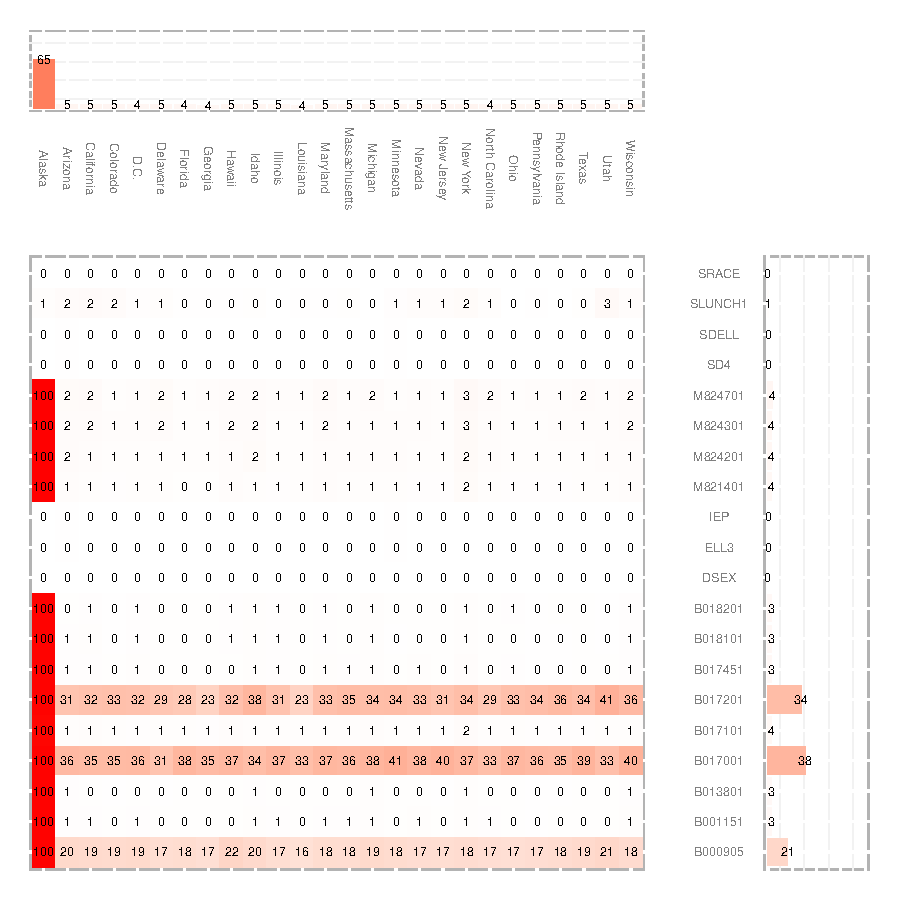
\includegraphics[height=.70\paperheight,keepaspectratio=true]{../Figures2009/g4math-missing.pdf} \\
	\end{center}
	For the logistic regression models the \texttt{MICE} \cite{mice} package was used to impute missing values.
\end{frame}

%%%%%%%%%%%%%%%%%%%%%%%%%%%%%%%%%%%%%%%%%%%%%%%%%%%%%%%%%%%%%%%%%%%%%%%%%%%%%%%%
\section{Analysis}

\subsection{Propensity Score Analysis using Stratification}

\begin{frame}[c]
	\frametitle{Loess Plot of Propensity Scores vs. Grade 4 Math}
	\begin{center}
	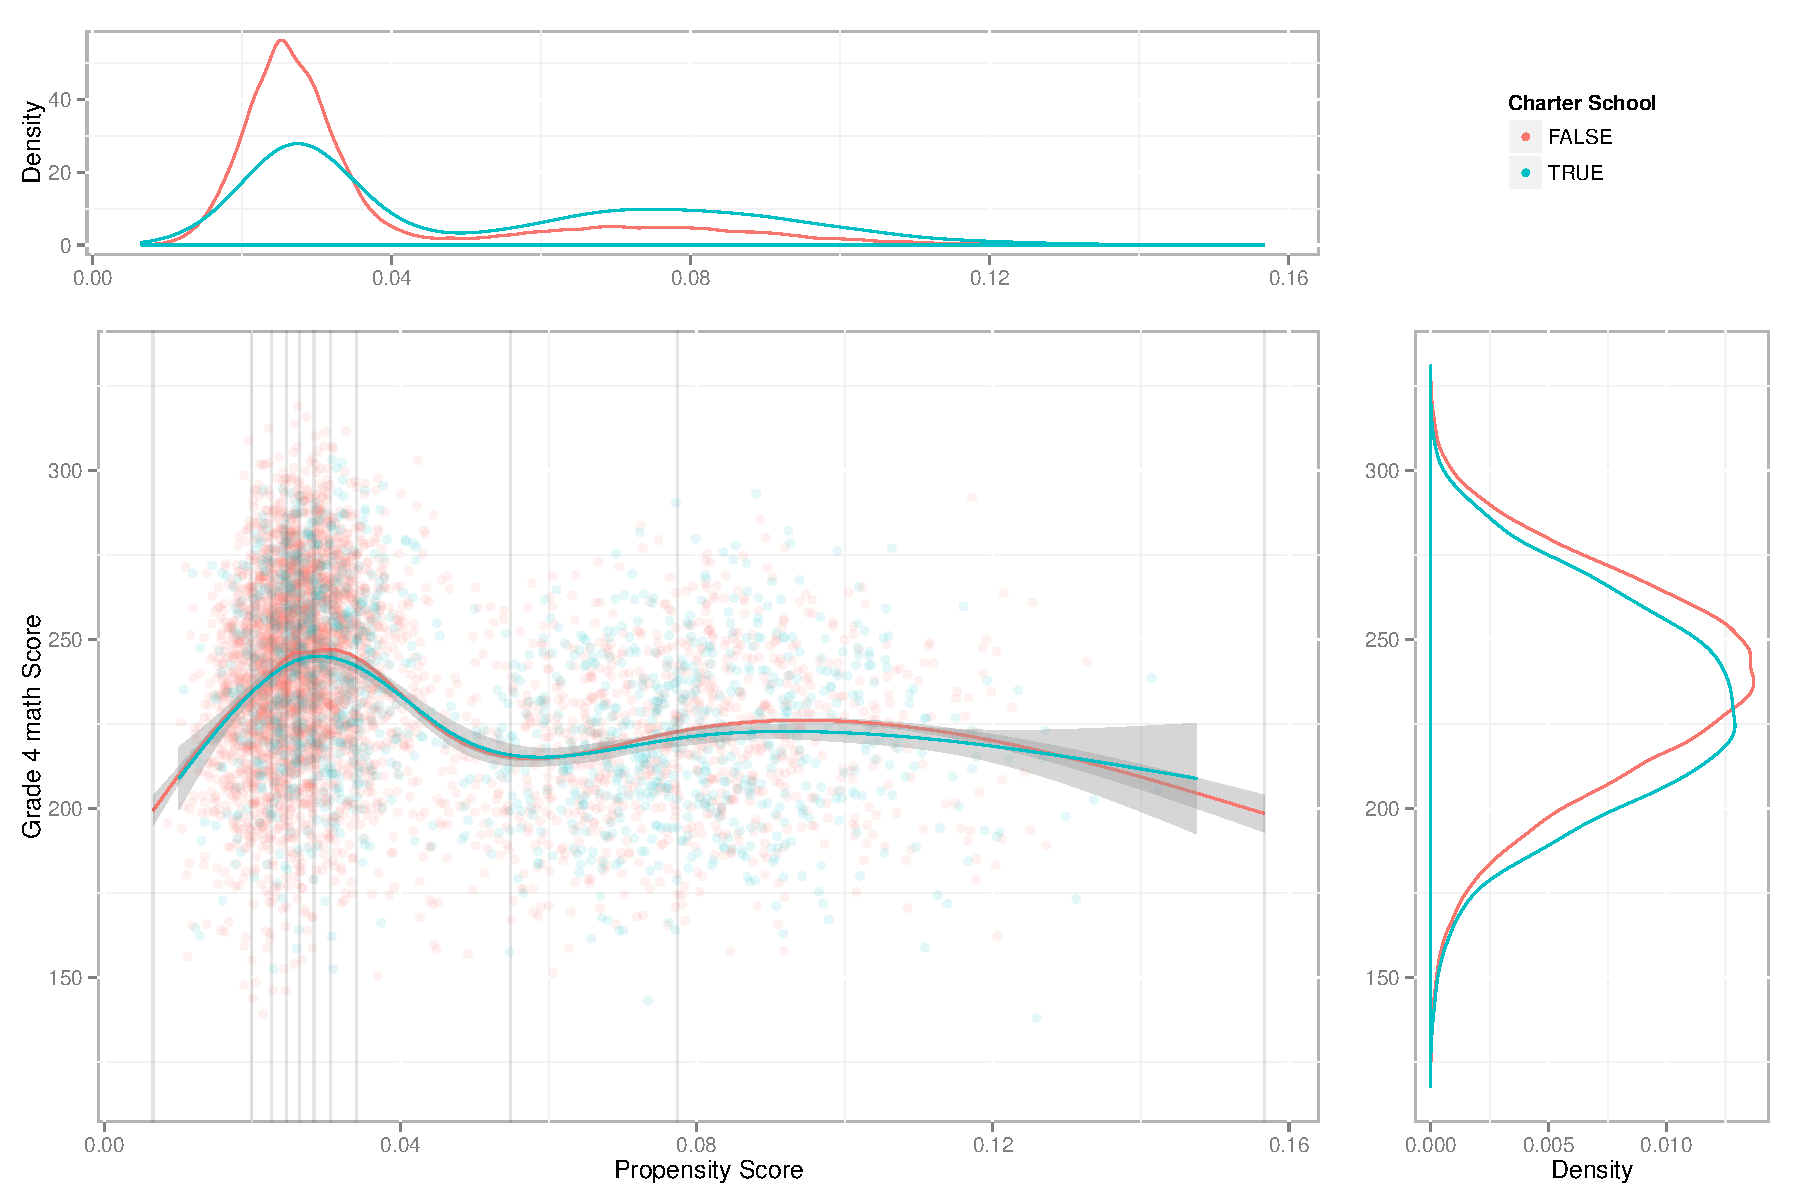
\includegraphics[width=0.9\paperwidth,keepaspectratio]{../Figures2009/g4math-loess}
	\end{center}
\end{frame}


\begin{frame}[c]
	\frametitle{PSA Assessment Plot: Grade 4 Math (Stratification)}
	\begin{center}
	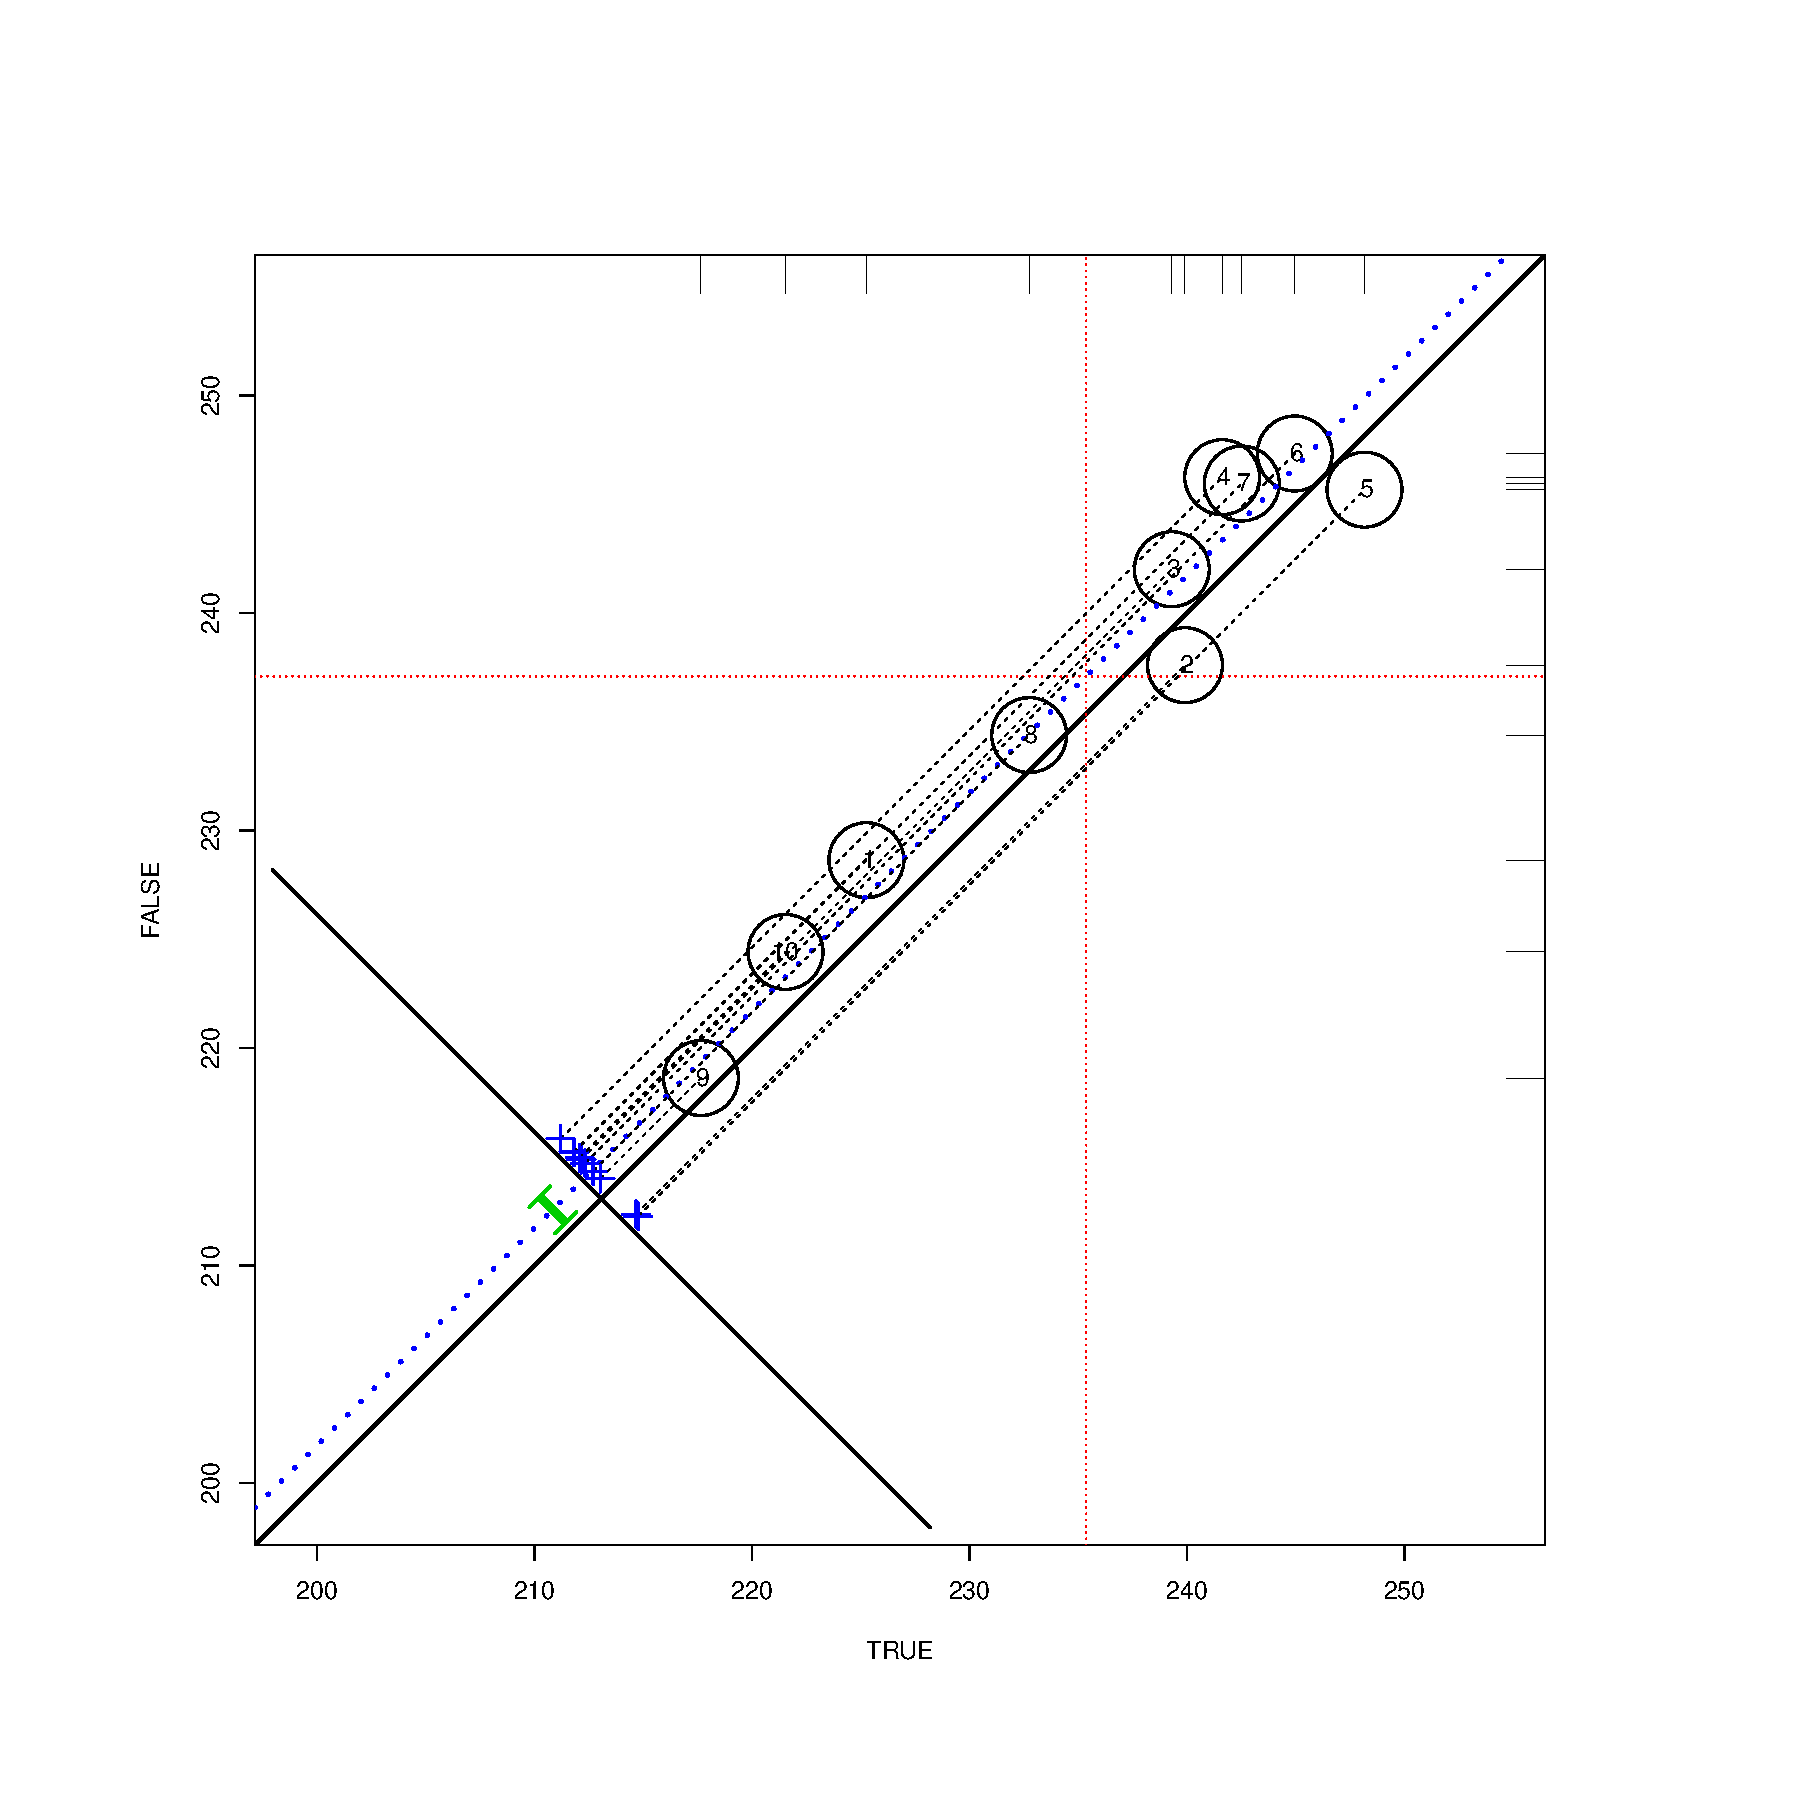
\includegraphics[height=0.9\textheight,keepaspectratio]{../Figures2009/g4math-circpsa10}
	\end{center}
\end{frame}

\begin{frame}[c]
	\frametitle{Boxplot of Means by Strata: Grade 4 Math}
	\begin{center}
	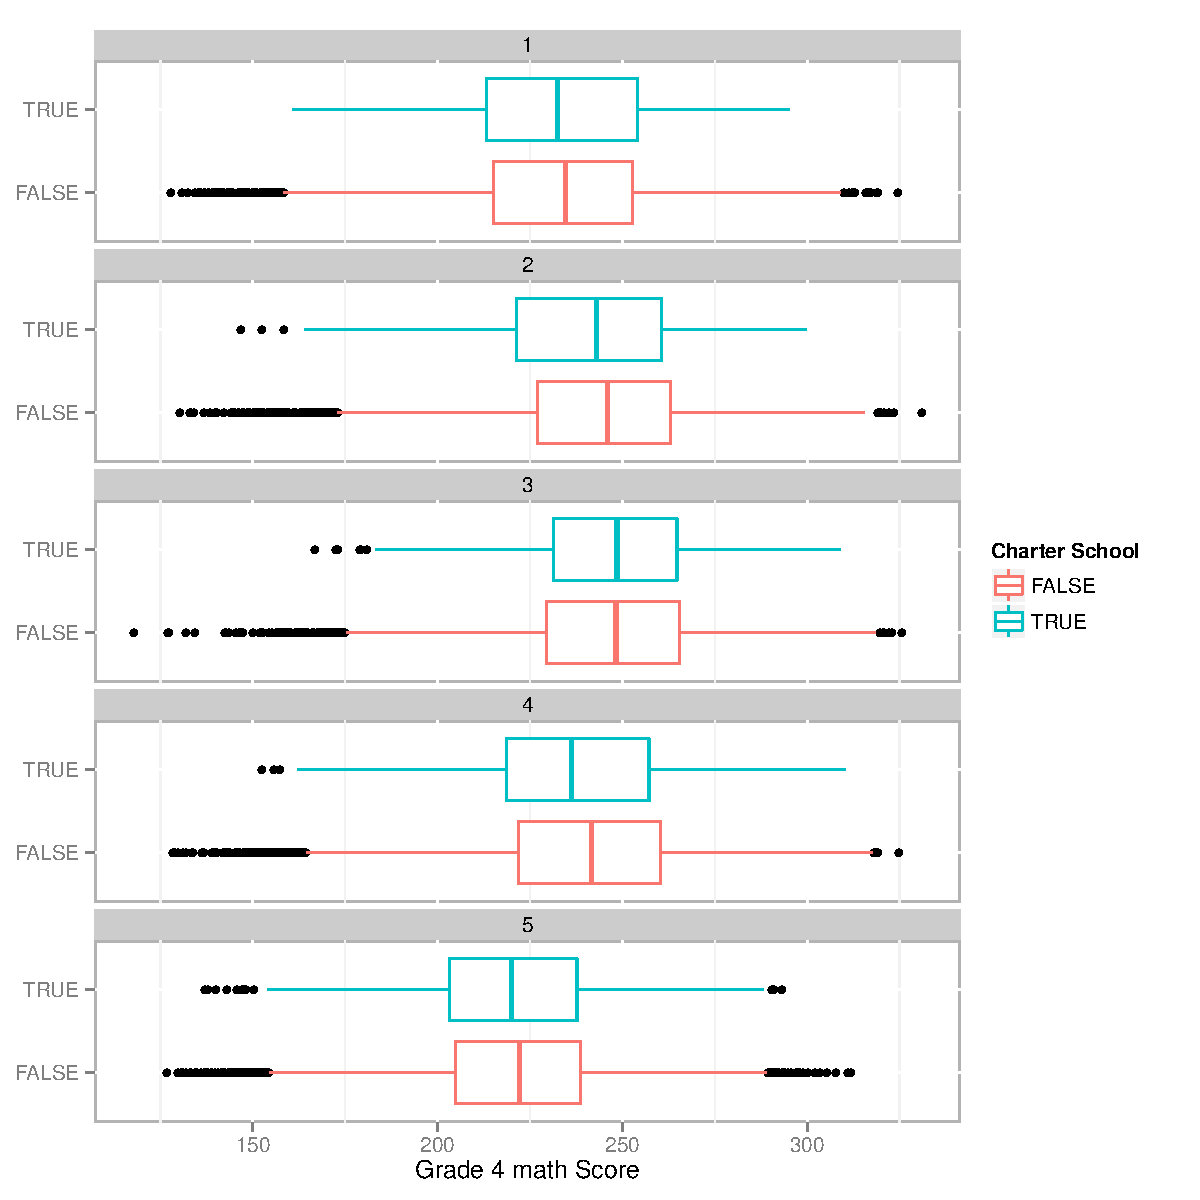
\includegraphics[height=0.86\textheight,keepaspectratio]{../Figures2009/g4math-strata5-boxplot}
	\end{center}
\end{frame}

\begin{frame}[c]
	\frametitle{Balance Plot: Grade 4 Math}
	\begin{center}
	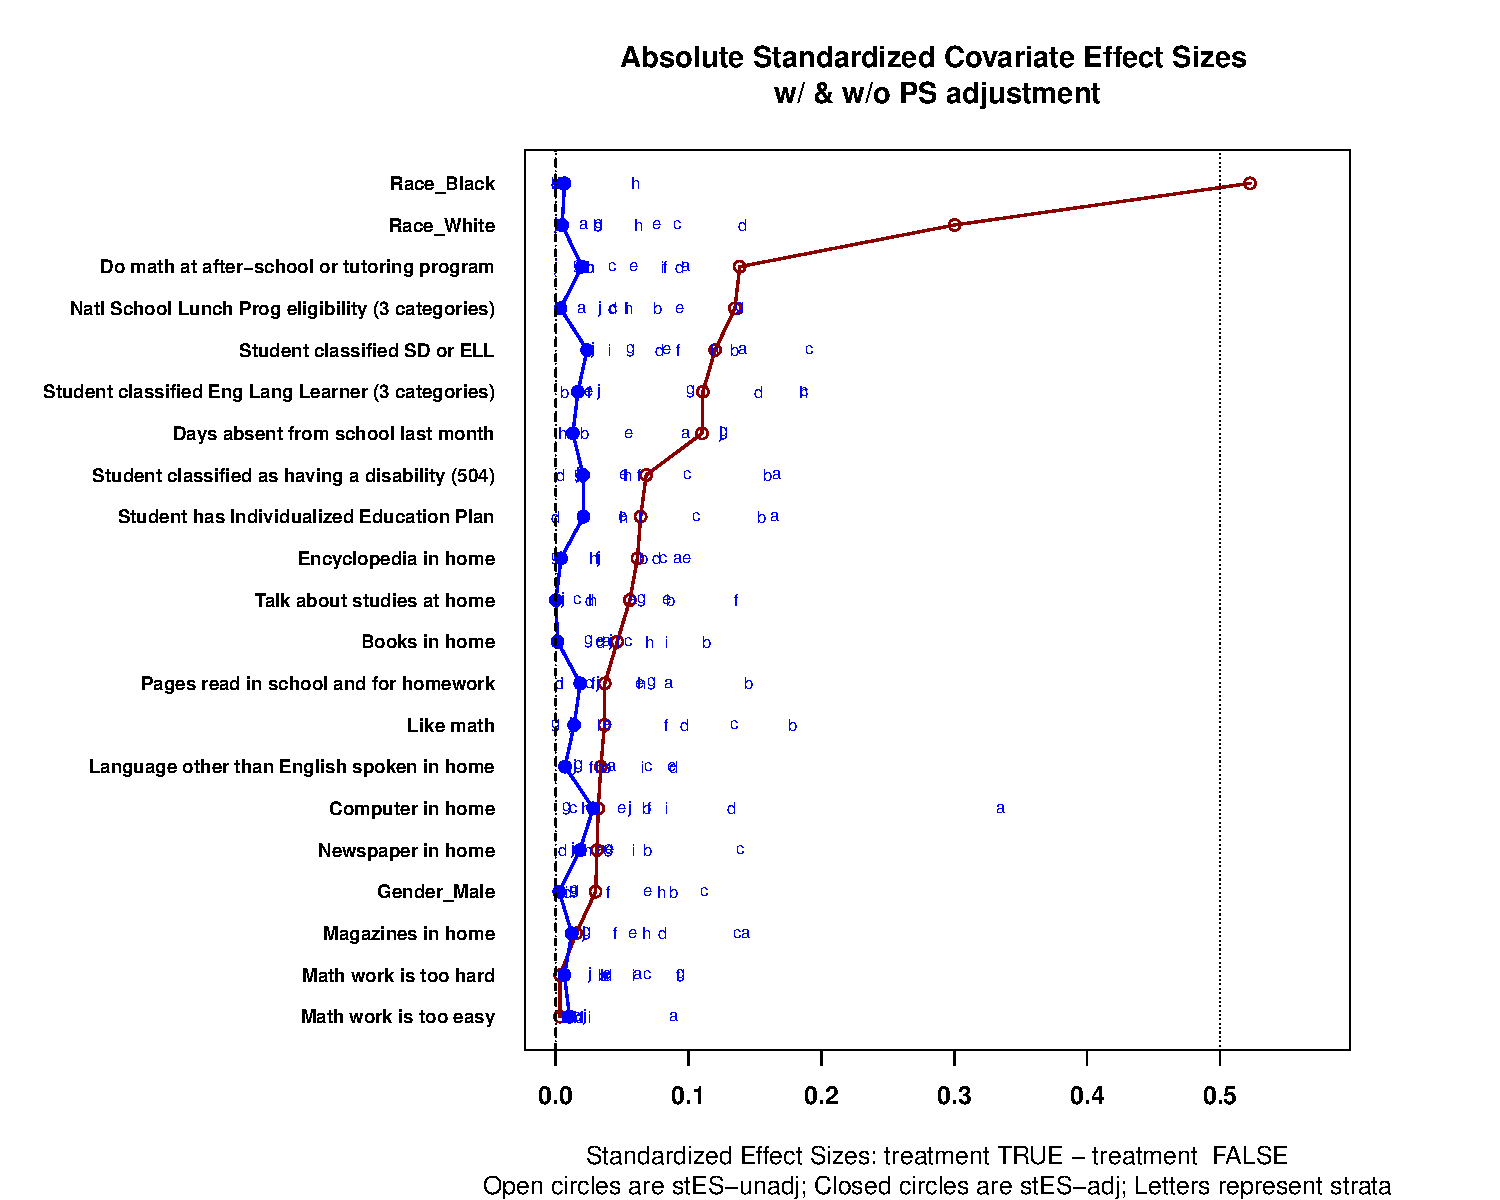
\includegraphics[height=0.86\textheight,keepaspectratio]{../Figures2009/g4math-lr-balance.pdf}
	\end{center}
\end{frame}


\subsection{Propensity Score Matching}

\begin{frame}[c]
    \frametitle{Propensity Score Matching}
    Partial exact matching using nearest neighbor was used using the \texttt{Matching} \cite{matching} package. For each charter school student:
    \ \\\ \\
    \begin{itemize}
    \setlength{\itemsep}{10pt}
        \item Traditional public school students in the same state with the same gender and ethnicity are located.
        \item Of those students, the student with the smallest difference in propensity scores is selected and paired with that charter school student.
    \end{itemize}
    \ \\\ \\
    Three match sets were estimated: one-to-one, one-to-five, and one-to-ten.
    \ \\\ \\
    For each match set, a dependent sample \textit{t}-test were used to estimate ATE.
\end{frame}

\begin{frame}
    \frametitle{The Relationship of Matched Pairs and Propensity Scores}
    \begin{center}
    	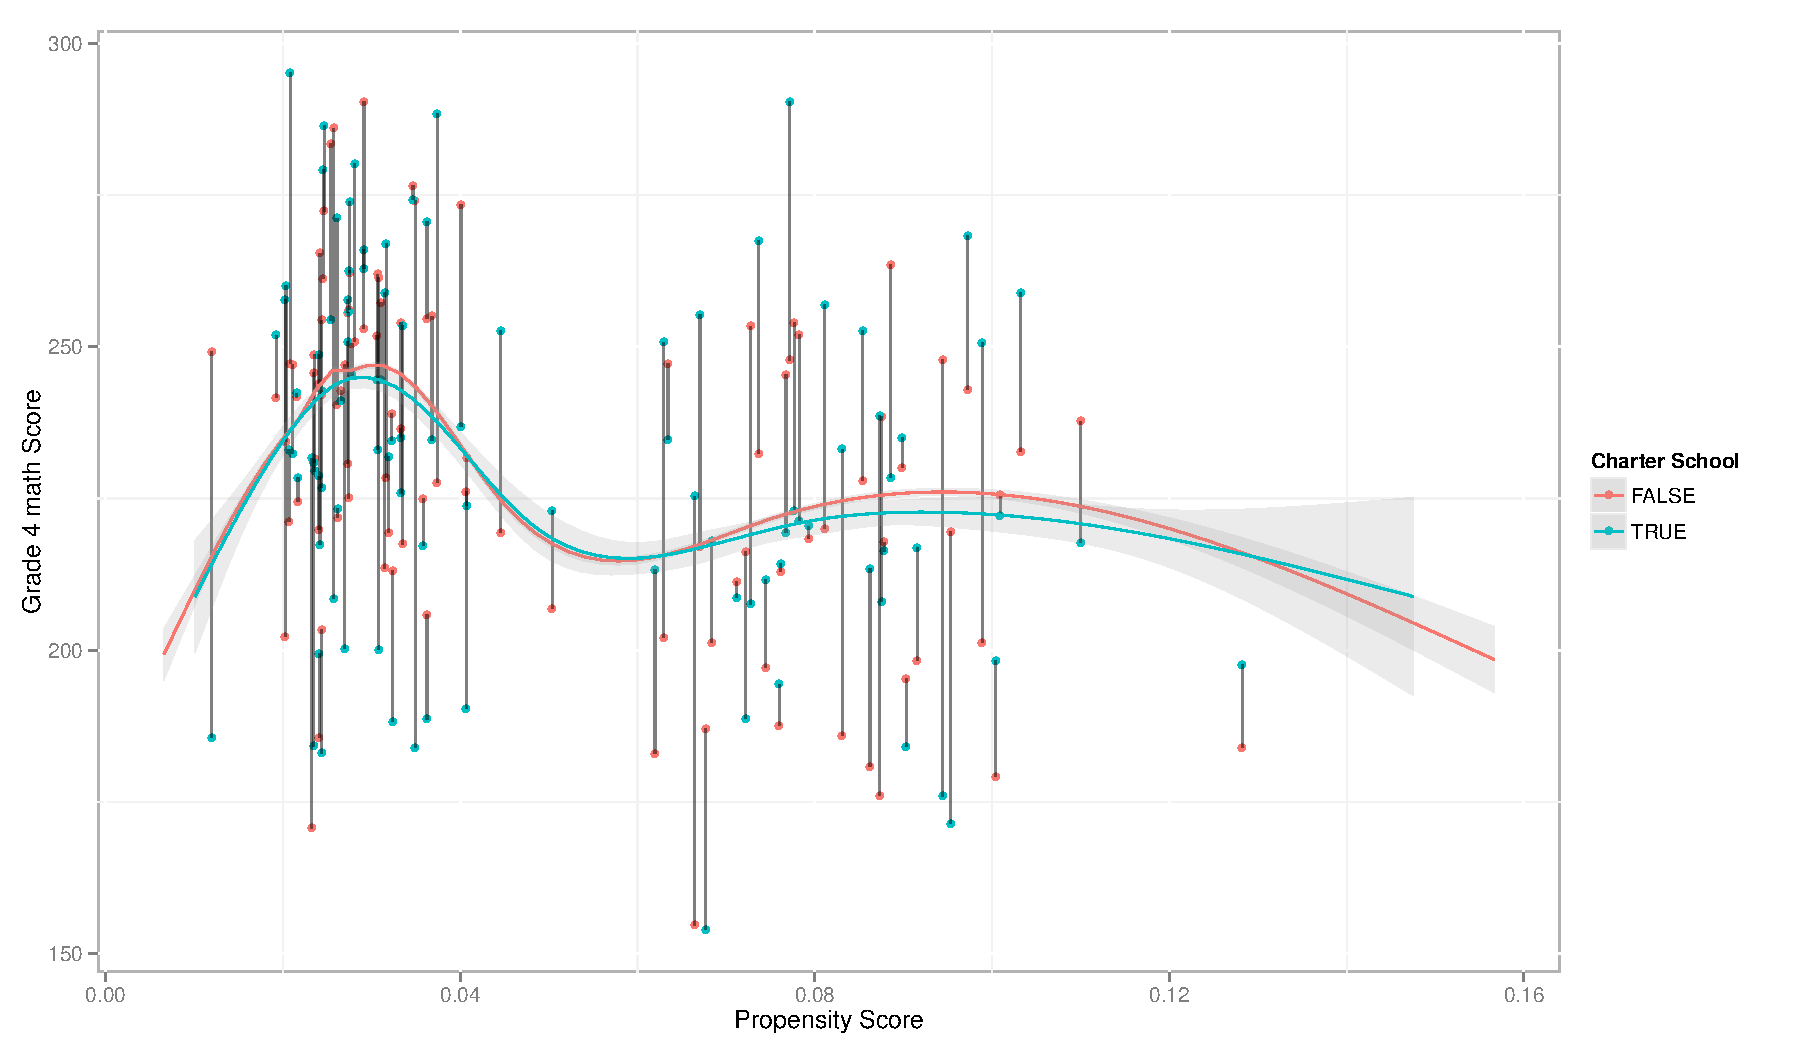
\includegraphics[width=\textwidth,keepaspectratio]{../Figures2009/g4math-loess-matching}
    \end{center}
\end{frame}


\begin{frame}[c]
    \frametitle{Propensity Score Matching Results}
\begin{table}[ht]
\centering
\begin{tabular}{lrrrrr}
  \hline Method & Charter & Public & ATE & \multicolumn{2}{c}{95\% CI} \\   \hline & \multicolumn{5}{c}{Grade 4 Math} \\ \cline{2-6} 
  Matching One-to-One & 231.22 & 231.18 & 0.00 & -1.12 & 1.20 \\ 
  Matching One-to-Five & 232.67 & 232.14 & 0.02 & -0.01 & 1.07 \\ 
  Matching One-to-Ten & 234.02 & 233.33 & 0.02 & 0.29 & 1.09 \\ 
    \hline & \multicolumn{5}{c}{Grade 4 Reading} \\ \cline{2-6} 
  Matching One-to-One & 212.88 & 211.82 & 0.03 & -0.30 & 2.41 \\ 
  Matching One-to-Five & 214.51 & 213.54 & 0.03 & 0.33 & 1.60 \\ 
  Matching One-to-Ten & 215.63 & 214.75 & 0.03 & 0.42 & 1.35 \\ 
    \hline & \multicolumn{5}{c}{Grade 8 Math} \\ \cline{2-6} 
  Matching One-to-One & 272.05 & 269.16 & 0.08 & 1.51 & 4.28 \\ 
  Matching One-to-Five & 274.85 & 273.46 & 0.04 & 0.72 & 2.06 \\ 
  Matching One-to-Ten & 276.21 & 274.08 & 0.06 & 1.63 & 2.62 \\ 
    \hline & \multicolumn{5}{c}{Grade 8 Reading} \\ \cline{2-6} 
  Matching One-to-One & 256.29 & 253.48 & 0.09 & 1.51 & 4.12 \\ 
  Matching One-to-Five & 258.19 & 256.24 & 0.06 & 1.33 & 2.58 \\ 
  Matching One-to-Ten & 258.93 & 256.82 & 0.06 & 1.65 & 2.57 \\ 
   \hline
\end{tabular}
\label{tab:overall}
\end{table}

\end{frame}


\subsection{Multilevel Propensity Score Analysis}

\begin{frame}[c]
	\frametitle{Covariate Heat Map for Stratification using Conditional Inference Trees}
	\begin{center}
	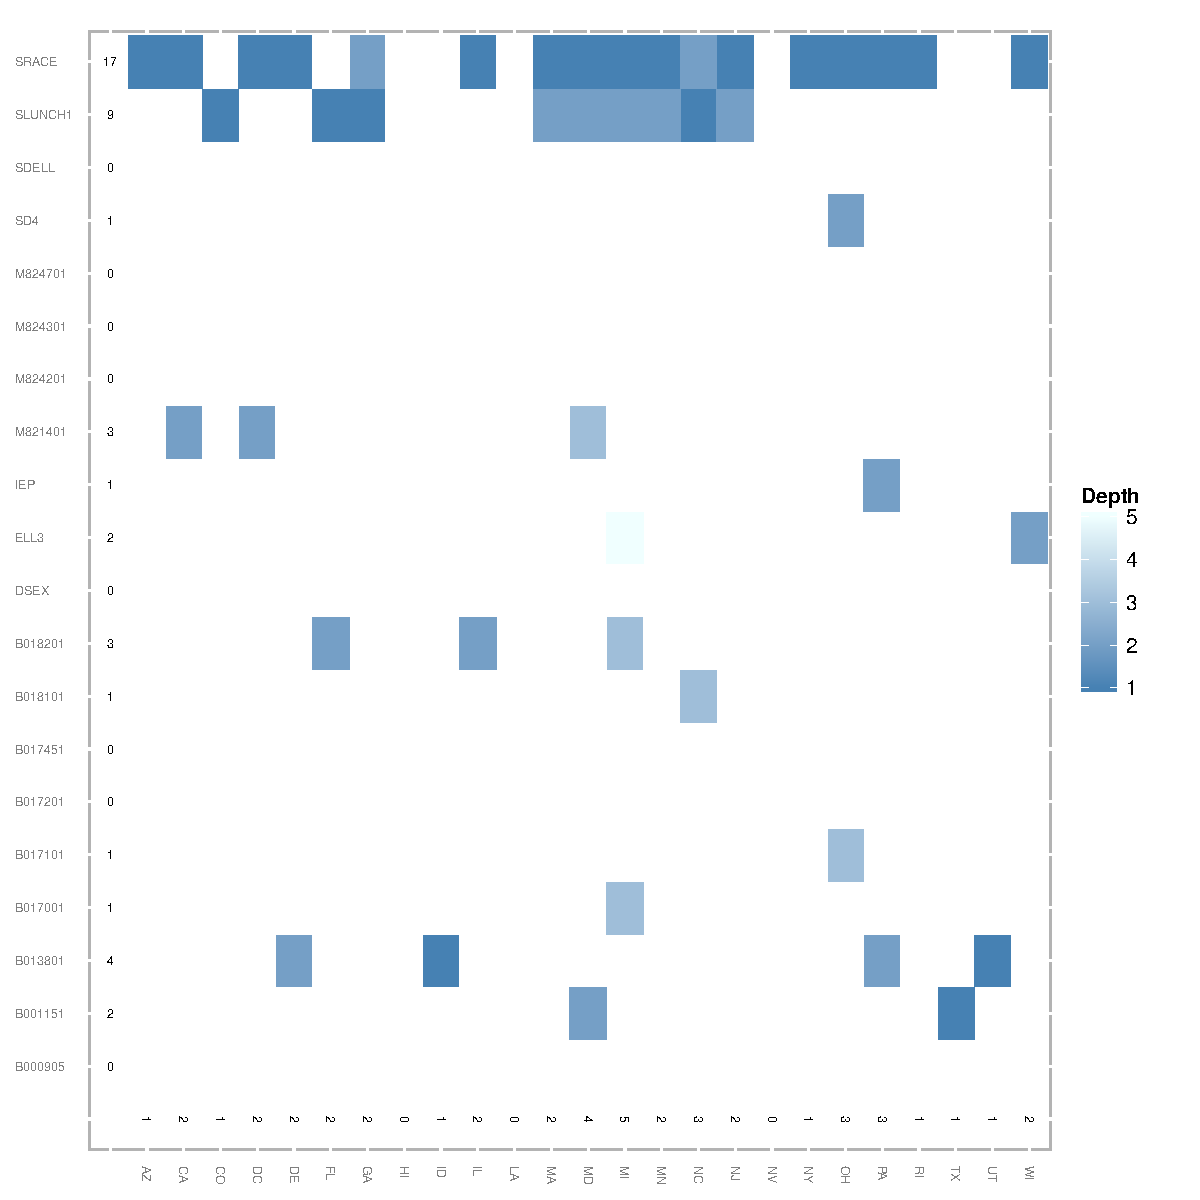
\includegraphics[width=\paperwidth,keepaspectratio]{../Figures2009/g4math-mlpsa-ctree-heat}
	\end{center}
\end{frame}


{ % Figure that fills the frame
    \setbeamertemplate{navigation symbols}{}
    \begin{frame}[plain]
        \begin{tikzpicture}[remember picture,overlay]
            \node[at=(current page.center)] {
                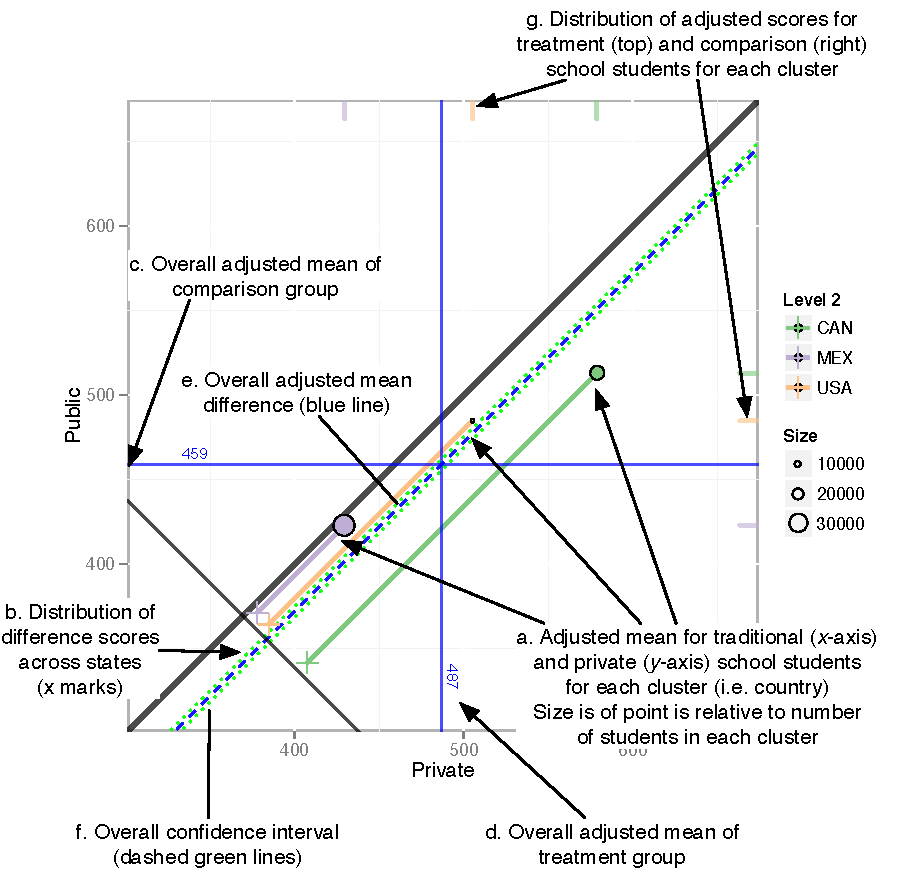
\includegraphics[height=\paperheight,keepaspectratio]{../Figures/AnnotatedCircPlot}
            };
        \end{tikzpicture}
     \end{frame}
}

\begin{frame}[c]
	\frametitle{Multilevel PSA Assessment Plot: Grade 4 Math}
	\begin{center}
	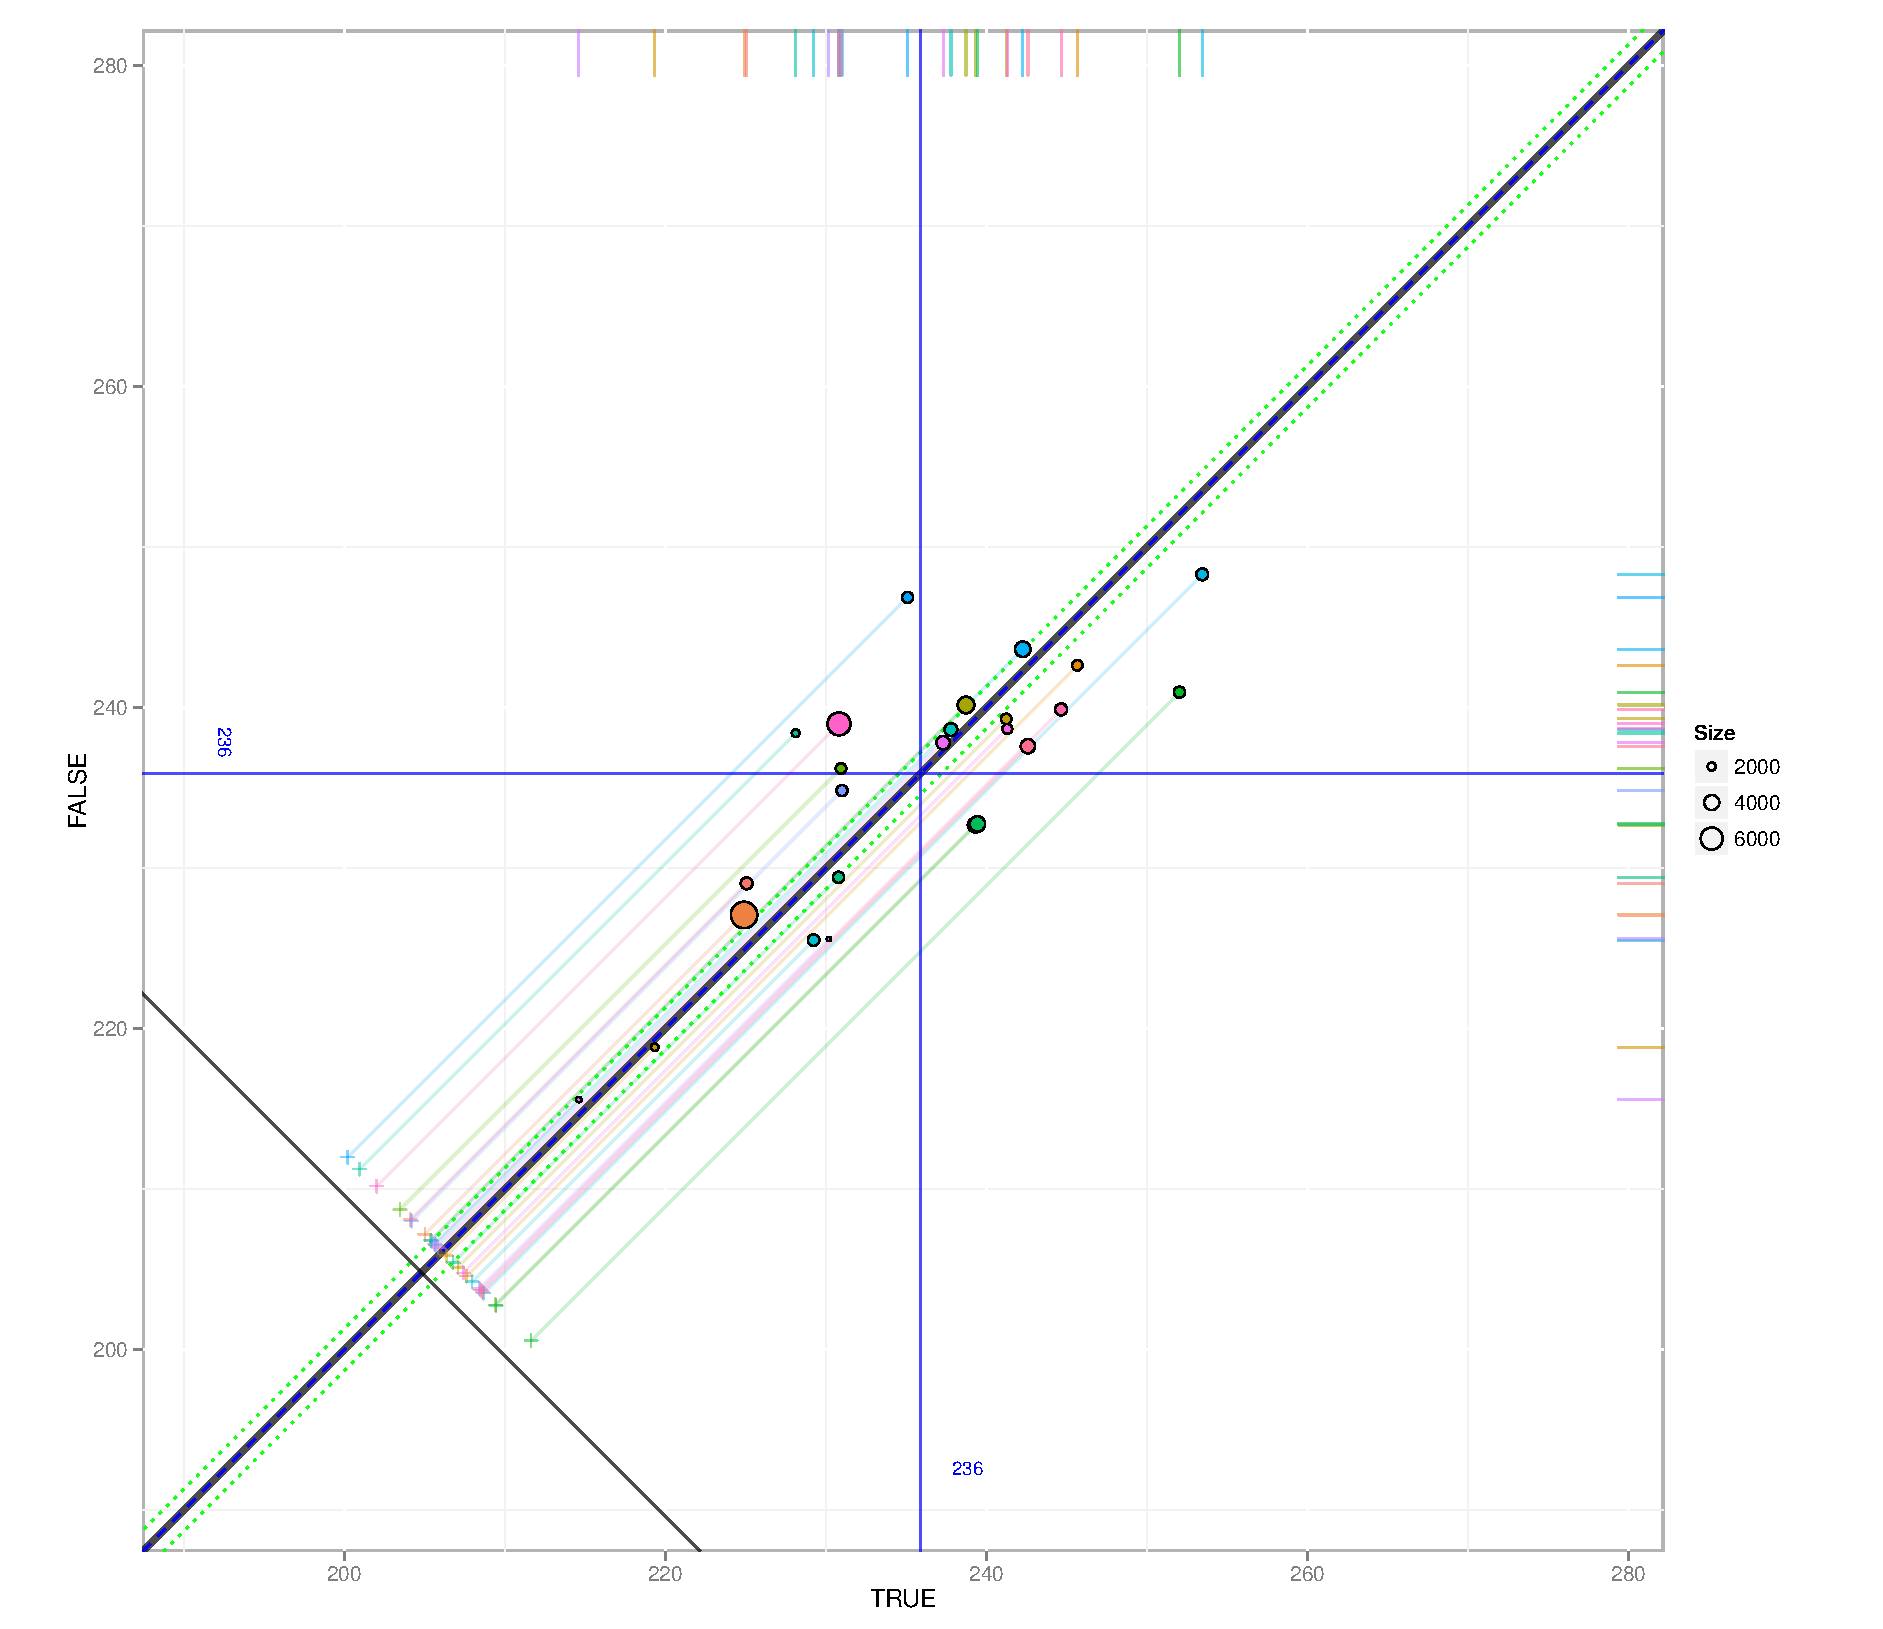
\includegraphics[height=\paperheight,keepaspectratio]{../Figures2009/g4math-mlpsa-ctree-circ}
	\end{center}
\end{frame}

\begin{frame}[c]
	\frametitle{Multilevel PSA Difference Plot: Grade 4 Math}
	\begin{center}
	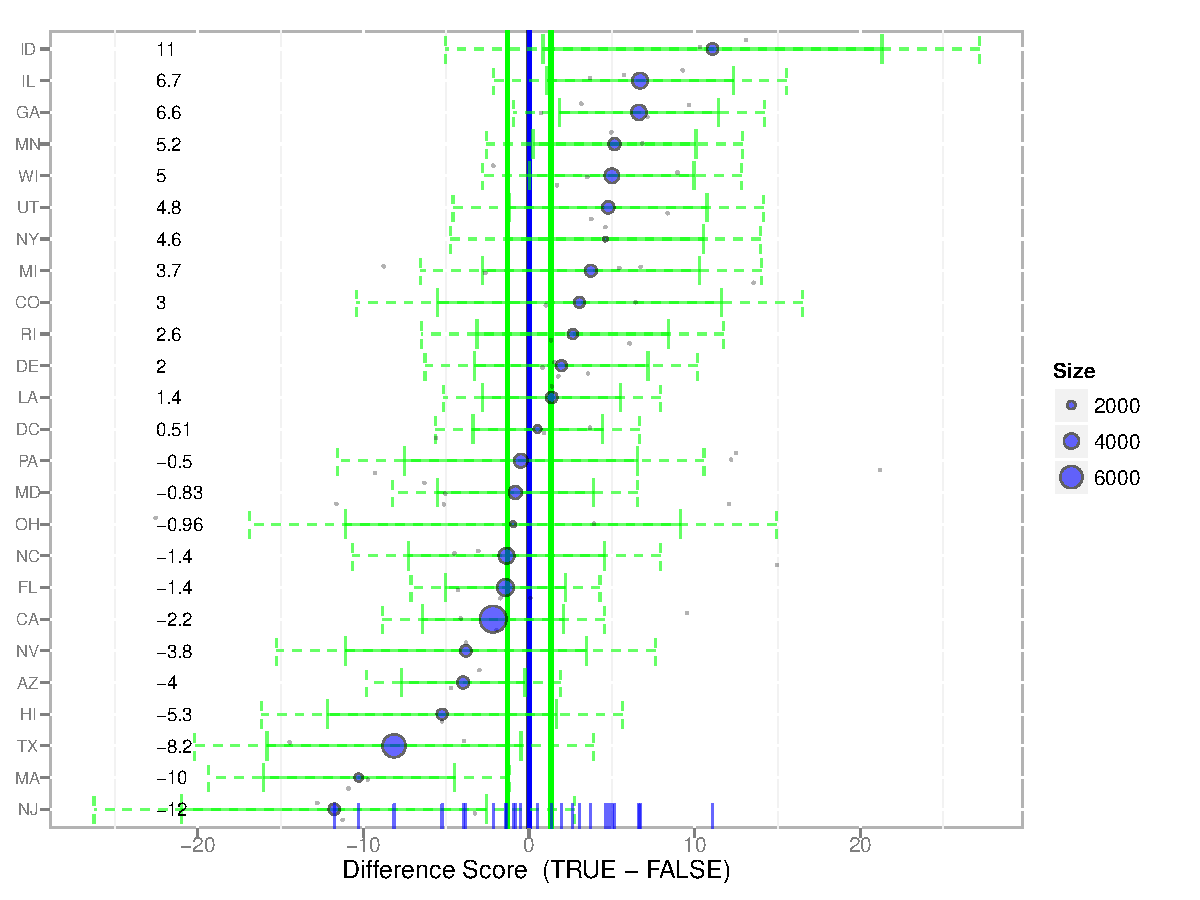
\includegraphics[height=\textheight,keepaspectratio]{../Figures2009/g4math-mlpsa-ctree-diff}
	\end{center}
\end{frame}

\begin{frame}[c]
	\frametitle{Multilevel PSA Balance Plot: Grade 4 Math}
	\begin{center}
	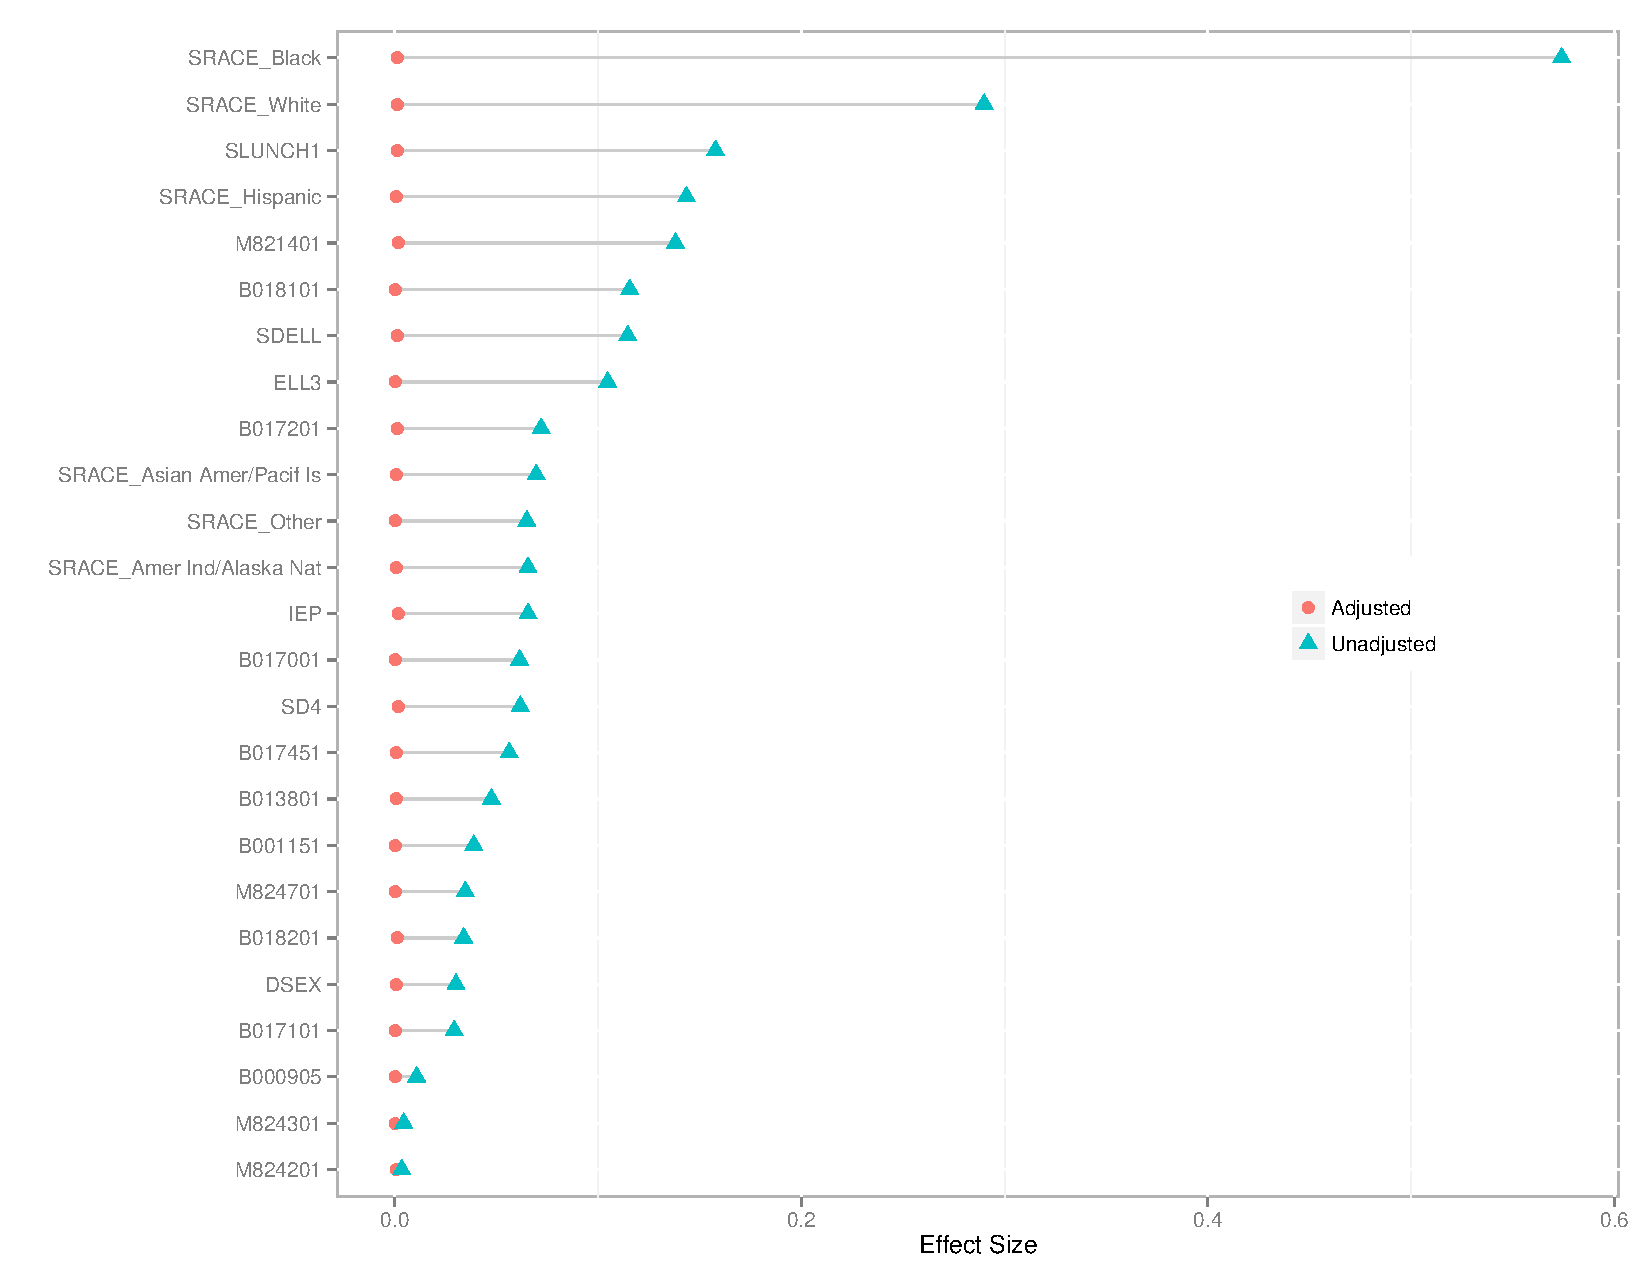
\includegraphics[height=\textheight,keepaspectratio]{../Figures2009/g4math-mlpsa-ctree-balance.pdf}
	\end{center}
\end{frame}

\begin{frame}[c]
    \begin{center}
    Lather, rinse, and repeat for grade 4 reading,\\grade 8 math, and grade 8 reading.
    \end{center}
\end{frame}


%%%%%%%%%%%%%%%%%%%%%%%%%%%%%%%%%%%%%%%%%%%%%%%%%%%%%%%%%%%%%%%%%%%%%%%%%%%%%%%%
\section{Overall Results \& Summary}

\begin{frame}[c]
	\frametitle{Scatterplot of Overall Adjusted Means (RQs 1 \& 2)}
	\begin{center}
	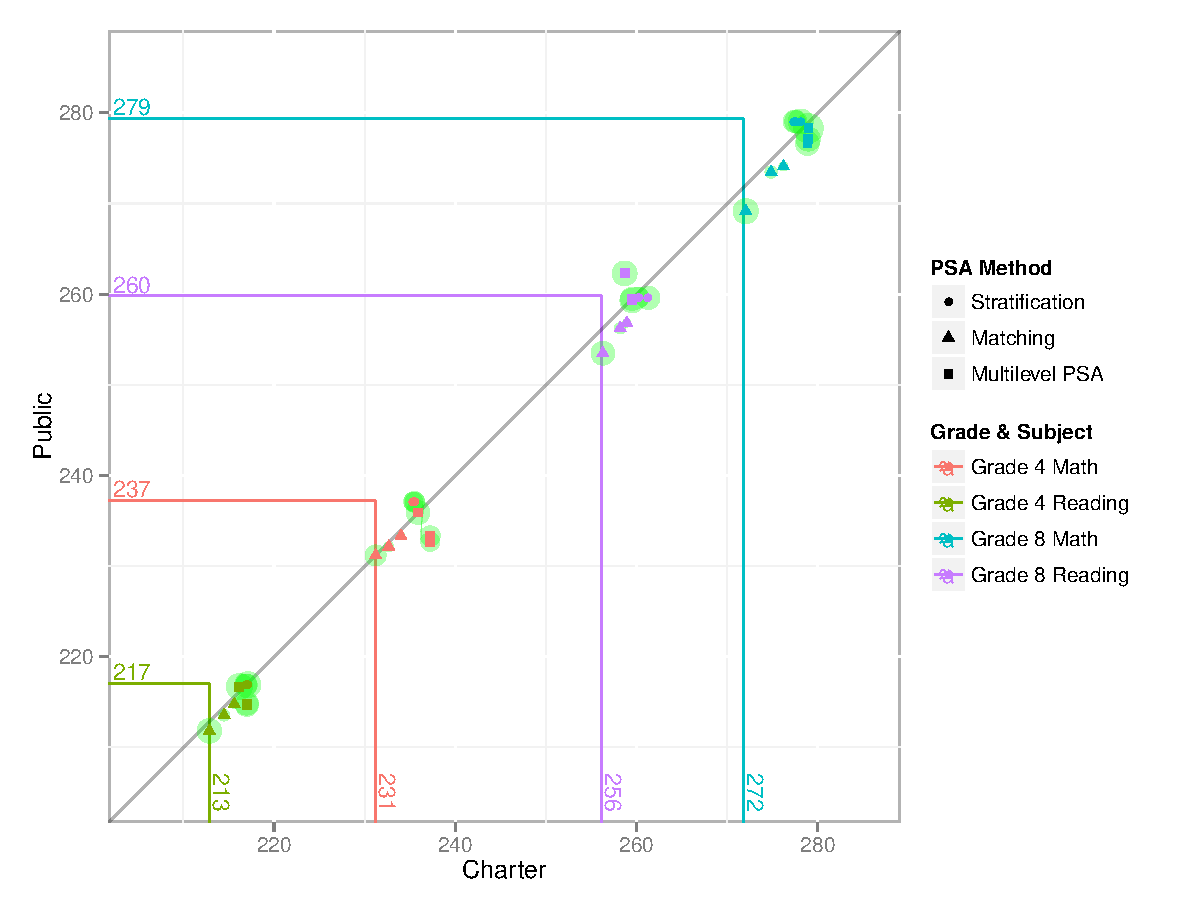
\includegraphics[width=0.85\paperwidth,keepaspectratio]{../Figures2009/OverallScatter}
	\end{center}
\end{frame}

\begin{frame}[c]
	\frametitle{Overall Effect Sizes (RQs 1 \& 2)}
	\begin{center}
	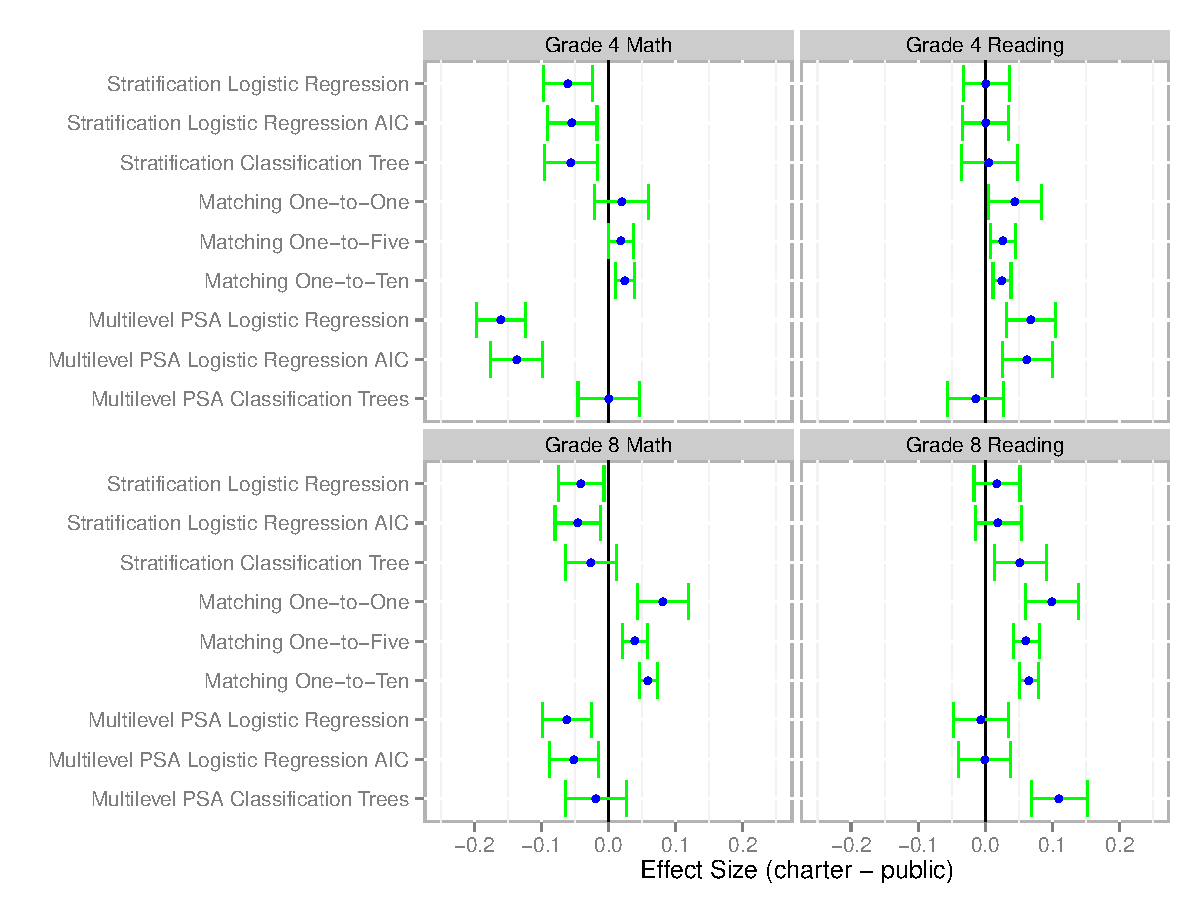
\includegraphics[width=0.85\paperwidth,keepaspectratio]{../Figures2009/Overall}
	\end{center}
\end{frame}

\begin{frame}[c]
	\frametitle{NAPCS Charter Law Scores vs. NAEP Effect Sizes (RQ 3)}
	\begin{center}
	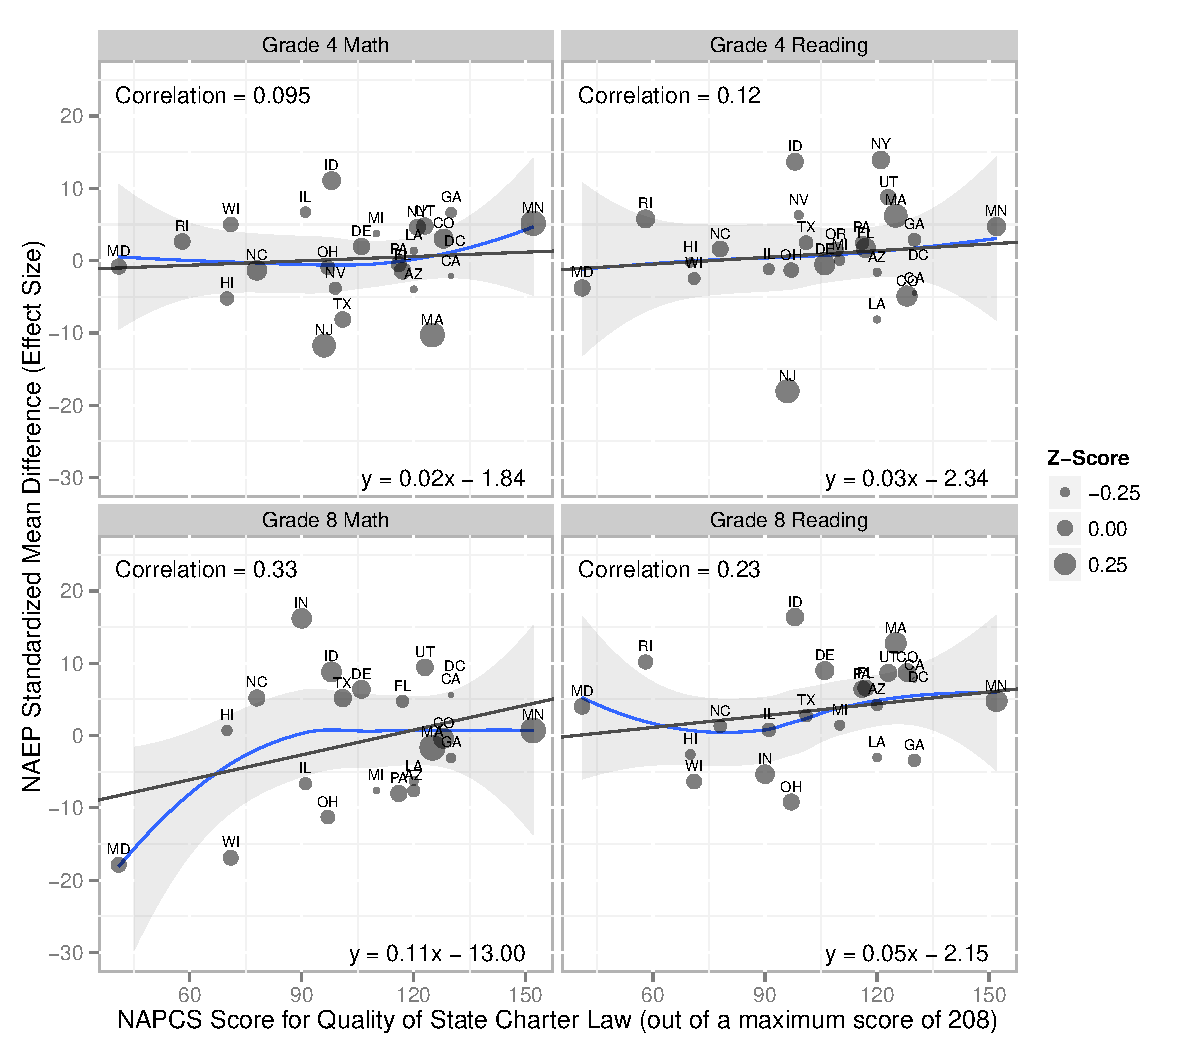
\includegraphics[height=.85\textheight,keepaspectratio]{../Figures2009/LawScoresVsNAEPDifferences}
	\end{center}
\end{frame}


%%%%%%%%%%%%%%%%%%%%%%%%%%%%%%%%%%%%%%%%%%%%%%%%%%%%%%%%%%%%%%%%%%%%%%%%%%%%%%%%
\section{Discussion \& Limitations}

\begin{frame}[c]
    \frametitle{Conclusions}
    \begin{itemize}
    \setlength{\itemsep}{10pt}
        \item There very little difference between the performance of charter and traditional public school in math and reading in grades 4 and 8 using NAEP as a measure of academic performance.
        \item The use of visualizations can be an important way to present results.
        \item The \texttt{multilevelPSA} R package is an important contribution to the PSA literature and is particularly useful in education research where many studies use data that is naturally multilevel (e.g. students within schools, within districts, within states).
        \item There is a small to moderate correlation between the quality of charter laws (as identified by NAPCS) and the outcomes from NAEP.
    \end{itemize}
\end{frame}

\begin{frame}[c]
    \frametitle{Limitations}
    \begin{itemize}
    \setlength{\itemsep}{10pt}
        \item This study only examines reading and math and does not consider other important subjects (e.g. history, science, the arts, etc.).
        \item There is variation in the quality and types of charter and traditional public schools, but they are considered together.
        \item Achieving balance using the multilevel PSA methods requires large sample sizes, especially for the logistic regression stratification methods.
        \item The analysis of the quality of charter laws is correlational. Further studies should look at how specific components that NAPCS has identified relate specifically to the performance of specific charter schools.
    \end{itemize}
\end{frame}


\begin{frame}[c]
	\frametitle{Resources}
	\begin{itemize}
    \setlength{\itemsep}{15pt}
		\item All of the R and \LaTeX{} code is available on Github (\url{http://github.com/jbryer/Dissertation}).
		\item \texttt{multilevelPSA} - An R package for the methods outlined here. Hosted at \url{http://github.com/jbryer/multilevelPSA} and documented at \url{http://jason.bryer.org/multilevelPSA/}.
		\item \texttt{naep} - An R package for accessing and analyzing NAEP data. This work was supported by Educational Testing Services (ETS) and the National Center for Education Statistics (NCES). Documentation is available at \url{http://jason.bryer.org/naep/}.
	\end{itemize}
\end{frame}


\begin{frame}[c]
	\LARGE{Thank You}\\
	\normalsize
	\ \\
	Jason Bryer (jason@bryer.org)\\
	\ \\
	\url{http://bryer.org}\\
\end{frame}


\begin{frame}[c,shrink=30]
    \nocite{HelmreichPruzek2009}
	\frametitle{References}
	\bibliographystyle{apacite}
	\bibliography{Bibliography}
\end{frame}


\begin{frame}
    \frametitle{20 Components of a Quality Charter Law}
    {\footnotesize
    \begin{columns}
        \begin{column}{0.5\textwidth}
            \begin{enumerate}
            \item No caps.
            \item A variety of public charter schools allowed.
            \item Multiple authorizers available.
            \item Authorizer and overall program accountability system required.
            \item Adequate authorizer funding.
            \item Transparent charter application, review, and decision-making processes.
            \item Performance-based charter contracts required.
            \item Comprehensive public charter school monitoring and data collection processes.
            \item Clear processes for renewal, nonrenewal, and revocation decisions.
            \item Educational service providers allowed.
            \item Fiscally and legally autonomous schools.
            \item Clear student recruitment, enrollment and lottery procedures.
            \end{enumerate}
        \end{column}
        \begin{column}{0.5\textwidth}
            \begin{enumerate}
            \setcounter{enumi}{12}
            \item Automatic exemptions from many state and district laws and regulations.
            \item Automatic collective bargaining exemption.
            \item Multi-school charter contracts and/or multi-charter contract boards allowed.
            \item Extra-curricular and interscholastic activities eligibility and access.
            \item Clear identification of special education responsibilities.
            \item Equitable operational funding and equal access to all state and federal categorical funding.
            \item Equitable access to capital funding and facilities.
            \item Access to relevant employee retirement systems.
            \end{enumerate}
            \cite{NAPCS2010a}
        \end{column}
    \end{columns}
    }
\end{frame}

\begin{frame}[c]
	\frametitle{Matrix Plot of NAPCS Quality of Charter Law Scores and NAEP Effect Sizes}
	\begin{center}
	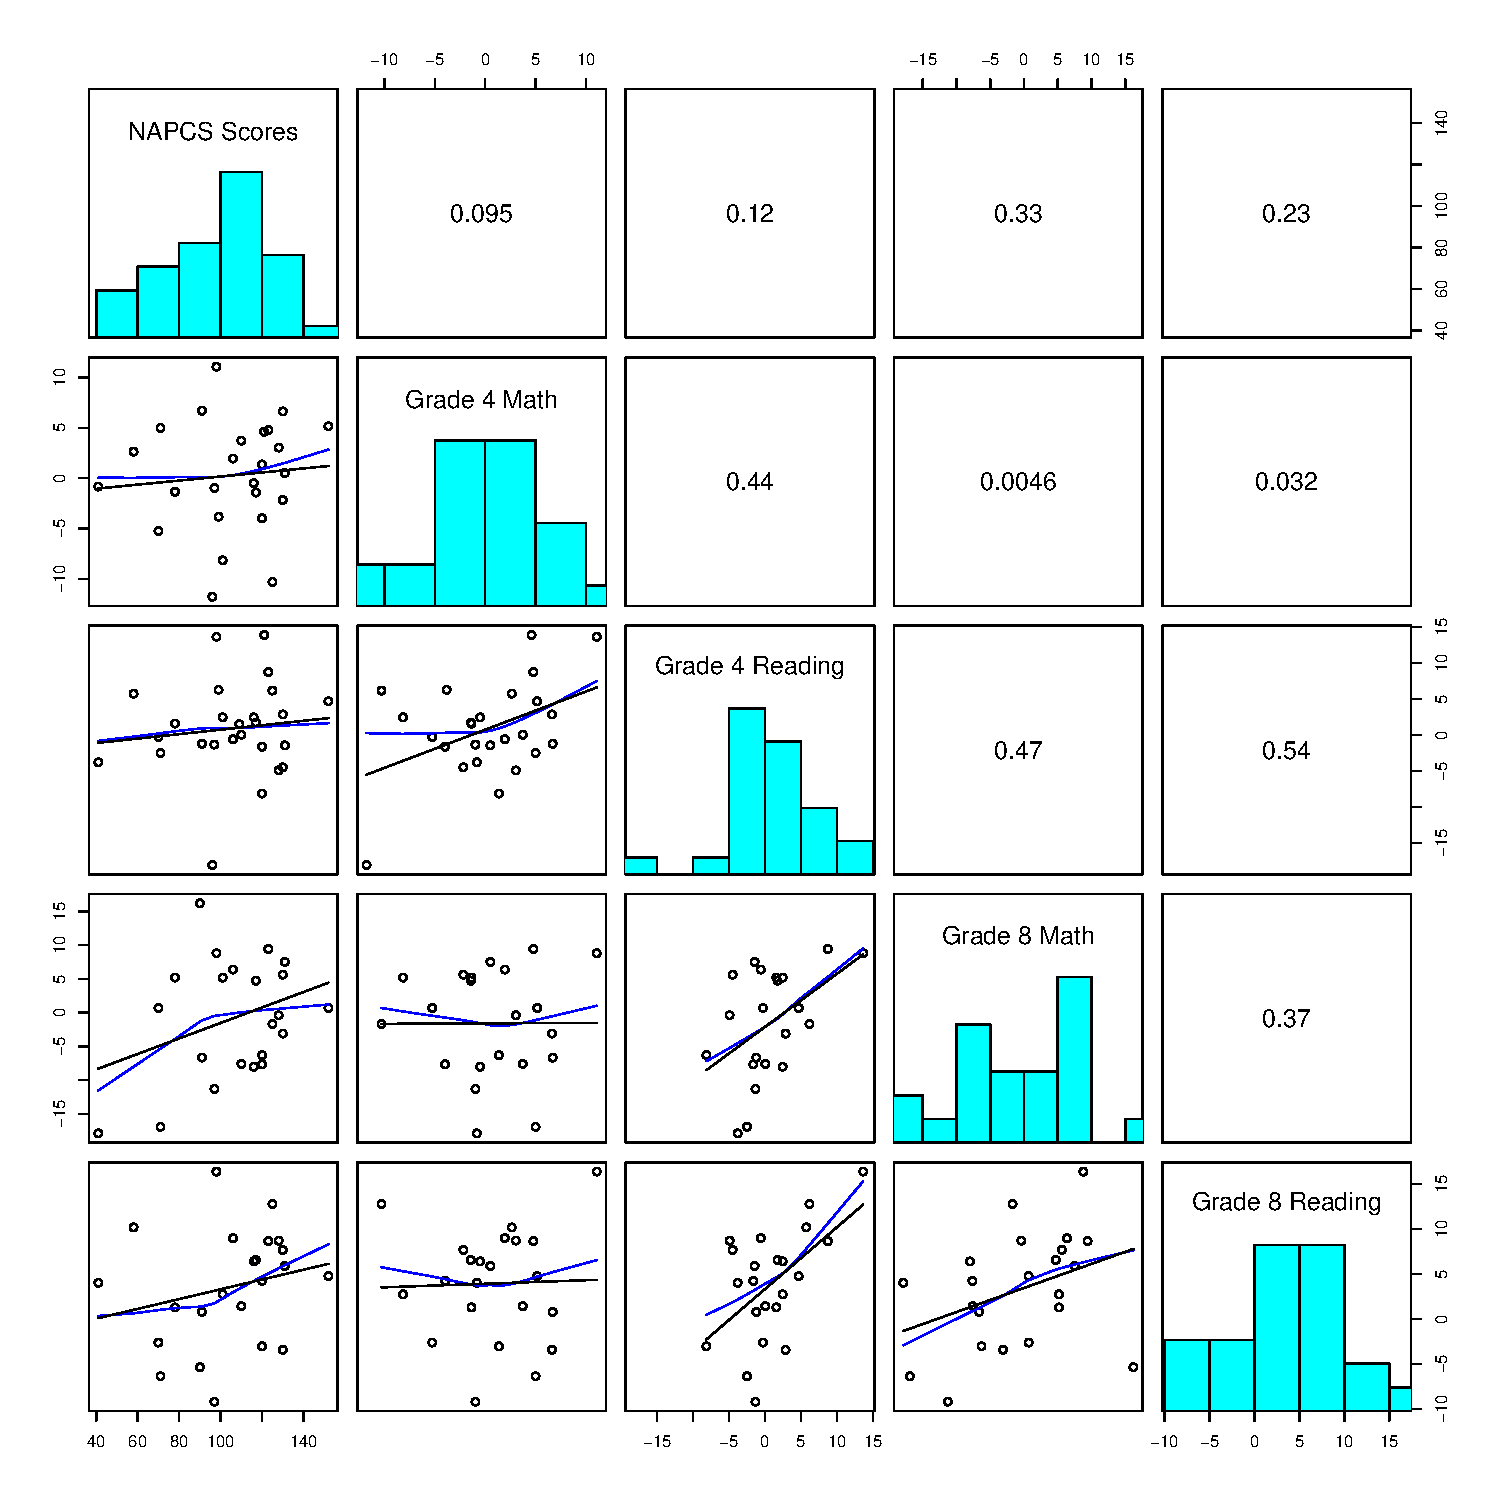
\includegraphics[height=.8\textheight,keepaspectratio]{../Figures2009/NAEPLawScoresMatrixPlot}
	\end{center}
\end{frame}


\end{document}
